%\section{Lensed waveguide}
%lensed_waveguide
In many articles it has been well discussed about the coupling between laser source and lensed fiber\cite{microlensese_to_fiber_coupling} and \cite{integrated_coupling _between_LD_SMF}. Authors of \cite{microlensese_to_fiber_coupling}  proved that  the coupling efficiency of their design reached maximum about $56\%$. \cite{integrated_coupling _between_LD_SMF} has also shown a minimum coupling loss less than $2$dB with application of a microlens. In compare with our previous works, our design could gain higher performance by the use of a microlens at the interface of the waveguide. For the fabrication it may be not easy to mount a microlens on a stript rib waveguide. But in \cite{lens_end_manufacture} the process sequence for fabricating the lens on the fiber end brings us the possibility to create a lens on a buried waveguide. In this section the coupling efficiency between TLF and the buried and lensed waveguide (or lensed waveguide) Fig. \ref{fig:lensed_waveguide} will be discussed. In this section the coupling efficiency between TLF and basic buried waveguide will at first be calculated as the reference for further discussing. Then we will engage the lensed waveguide and the effect of changing the lens geometric ($h$ and $R$) parameters of the lensed waveguide. 
\begin{figure}[!ht]
\centering
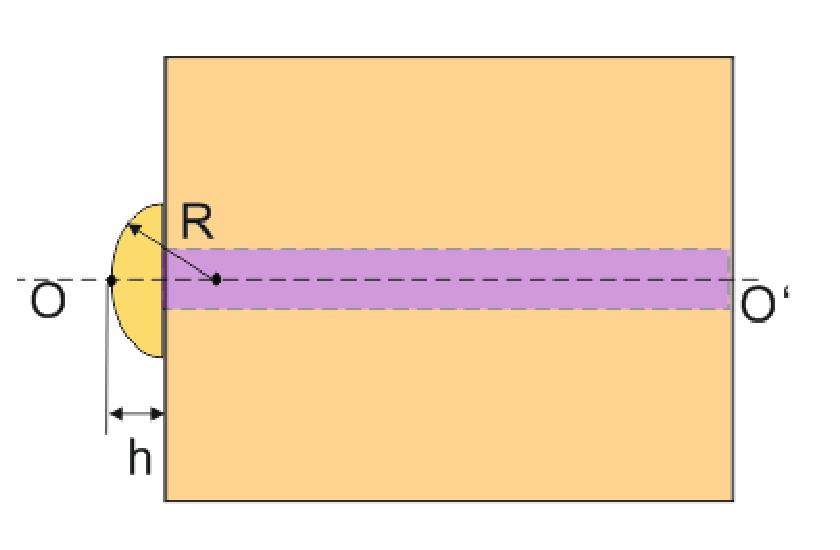
\includegraphics[width=0.7\textwidth]{bilder/lensed_waveguide}
\caption{Schema of a lensed buried waveguide.}
\label{fig:lensed_waveguide}
\end{figure}